\chapter{Modelling Game Dynamics with Markov Chains}
Building upon the empirical insights into Snakes and Ladders game dynamics from agent-based simulations in Chapters 2 and 3, this chapter introduces a complementary analytical approach: a Markov Chain model. This chapter details construction and validation of this model to predict expected game length, win probabilities, and come to a steady-state distributions. Crucially, this Markovian framework serves to analytically verify the empirical findings from our simulations.

\section{What are Markov Chains}
A Markov chain is a mathematical construct describing a system transitioning between discrete states in a sequential, chain-like manner \autocites{dusautoyWorldEightyGames2024}. The defining characteristic, and analytical power, of a Markov chain lies in its ‘memoryless’ property: future state transitions depend solely on the current state, irrespective of the sequence of states that preceded it. In the context of Snakes and Ladders, we conceptualise each tile on the board as a distinct state. The probabilistic transition from one tile to the next is governed by the outcome of a dice roll, rendering the game dynamics amenable to Markovian analysis.

By adopting this framework, we can mathematically represent the inherent randomness of dice rolls and the deterministic rules of snake and ladder placements. This allows us to move beyond empirical observation and offers a powerful means of validating and extending our simulation-based research.

\subsection{Fundamental Concepts}
To ensure clarity and precision in our model description, it is essential to define the core concepts underpinning our Markovian approach:
\begin{enumerate}
	\item \textbf{States:} Each tile on the Snakes and Ladders board, indexed from 1 to $BoardSize$, is defined as a unique state within our Markov model. State 1 represents the starting position, and state $BoardSize$ corresponds to the final tile, the absorbing goal state.
	\item \textbf{Transitions:} Game progression is modelled as probabilistic transitions between these states. Transitions occur in discrete steps, driven by dice rolls. Each roll of a fair six-sided die produces an outcome $k \in \{1, 2, 3, 4, 5, 6\}$, each with an equal probability of $\frac{1}{6}$. Adding this outcome to the current tile number determines a tentative next position, subject to board boundaries and entity adjustments.
	\item \textbf{Absorbing State:} The final tile, state $BoardSize$, is designated as an absorbing state. Once a player reaches or surpasses tile $BoardSize$, the game concludes, and the player remains in this state indefinitely. This is mathematically represented by a self-loop in the transition matrix, with a probability of 1.
	\item \textbf{Memorylessness (Markov Property):} The defining ‘memoryless’ property dictates that the probability of transitioning to any future state depends exclusively on the current state. The history of previous moves or states is irrelevant. This assumption is valid for Snakes and Ladders, as each dice roll and subsequent move are probabilistically independent of prior game events.
\end{enumerate}

\subsection{Constructing the Transition Matrix}
The core of our Markov model is the transition matrix, $P$, a square matrix of size $(\text{BoardSize}-(N_s + N_l)) \times (\text{BoardSize}-(N_s + N_l))$. Each entry $P(i,j)$ quantifies the probability of transitioning from state $i$ to state $j$ in a single turn. To maintain the state space and focus on board position transitions, we do not treat snake heads or ladder bases as distinct states \autocite{dusautoyWorldEightyGames2024}. An $\text{BoardSize}\times \text{BoardSize}$ matrix may be used to study the same phenomena, but since the probability of staying on tiles with entity triggers is going to remain the same as landing on the other terminal tile, therefore, we reject these tiles. This aids the computation as well, since Matrix Multiplication using the Naive Algorithm has a time complexity of $O(N^3)$ and would scale tremendously as we scale board sizes. For baseline analysis within this chapter, we configure the board with 10 snakes ($N_S$) and 10 ladders ($N_L$), with their lengths assigned randomly using the fixed start and end points methodology detailed in Chapter 2.

For each non-absorbing state $i < N$:
\begin{enumerate}
	\item \textbf{Dice Roll Simulation:} We simulate the roll of a fair six-sided die, generating an outcome $k \in \{1, 2, 3, 4, 5, 6\}$, each with a probability of $\frac{1}{6}$.
	\item \textbf{Tentative Movement:} A tentative next state is calculated by adding the dice roll outcome $k$ to the current state $i$ (Constrained to Chapter 2's set up).
	\item \textbf{Entity-Based Adjustment:} We then check if the tentative next state coincides with the start of a snake or the base of a ladder, based on the pre-defined board layout. If so, the state is immediately updated to the corresponding snake tail or ladder top, respectively.
	\item \textbf{Probability Assignment:} For each dice outcome $k$, the transition probability ($\frac{1}{6}$) is added to the matrix entry $P(i, j)$, where $j$ represents the final state reached after all movement and entity-based adjustments.
\end{enumerate}

For the absorbing state BoardSize, the transition matrix row is configured to represent absorption: $P(\text{BoardSize, BoardSize}) = 1$, and $P(\text{BoardSize}, j) = 0$ for all $j \neq \text{BoardSize}$. This ensures that once the final state is reached, the probability of transitioning to any other state is zero. For all other (non-absorbing states) $i<\text{BoardSize}$, the transition probabilities are determined directly based on the board layout. For each state $i$ and each possible dice roll outcome, we directly determine the next state $j$ based on the board layout. The $P_{ij}$ is then simply the count of dice rolls that lead to $j$ divided by 6.

Notationally, for non-absorbing states $i < N$, the transition probability is expressed as:
\[
P(i, j) = \sum_{k=1}^{6} \frac{1}{6} \cdot \mathbf{1}\{f(i,k) = j \}
\]
where $f(i,k)$ is a function encapsulating the game's movement rules: it computes the next state $j$ reached from state $i$ after rolling $k$, incorporating boundary reflections and snake/ladder adjustments. The indicator function $\mathbf{1}\{\cdot\}$ evaluates to 1 if the condition is true, and 0 otherwise.

For the absorbing state $N$, the transition probabilities are deterministic:
\[
P(N, N) = 1, \quad P(N, j) = 0 \quad \forall j \neq N.
\]
This formulation guarantees that each row of the transition matrix sums to unity, a fundamental property of stochastic matrices and Markov chains \autocite{dusautoyWorldEightyGames2024}.

\section{Analytical Derivation of Game Metrics}

With the transition matrix constructed, we can analytically derive key game metrics using matrix-based methods. Specifically, we leverage the concept of the fundamental matrix to calculate expected game turns and estimate win probabilities.

\subsection{Fundamental Matrix and Expected Turns}

To calculate the expected number of turns to reach the absorbing state, we first partition the transition matrix $P$ into submatrices corresponding to transient (non-absorbing) and absorbing states. Let $Q$ be the submatrix representing transitions between transient states, and $R$ be the submatrix for transitions from transient to absorbing states. The fundamental matrix $N$, central to our analysis, is then computed as:
\[
N = (I - Q)^{-1}
\]
where $I$ is the identity matrix of the same dimension as $Q$. The entry $N(i, j)$ of the fundamental matrix provides the expected number of times the system visits transient state $j$ before absorption, starting from transient state $i$.

The expected number of turns, $t$, to reach the absorbing state from a starting state $i$ is derived by summing the entries in the $i^{th}$ row of the fundamental matrix $N$ and multiplying by a column vector of ones, $\mathbf{1}$:
\[
t_i = (N \cdot \mathbf{1})_i = \sum_{j} N(i, j)
\]
For a standard Snakes and Ladders game starting at state 0, the expected number of turns to reach the final tile is:
\[
t = t_0 = \sum_{j} N(0, j)
\]

This sum represents the total expected number of steps spent in transient states before absorption, effectively quantifying the average game duration in turns \autocites{dusautoyWorldEightyGames2024}.

For example, for a 2x2 board, with 4 tiles labelled 1 through 4 and using a 2-sided die (i.e. only move 1 or 2 tiles ahead). The board has a snake going from tile 3 back to tile 1, and a ladder going from tile 2 to tile 4. The probability of going from tile 1 to tile 2 or 3 becomes 1/2, but since tiles 1 and 2 are entity triggers, they are removed from the transition matrix. The transition matrix thus for the same is of the form:
$$P = \begin{pmatrix}
	\frac{1}{2} & \frac{1}{2}\\
	0 & 1
\end{pmatrix}$$
Here, the first row, represents the probability of going from tiles 1 to 1 and 1 to 4, and the second row shows the probability of going from tile 4 to tile 1 and finally the absorbing state which goes from tile 4 to 4 with absolute certainty.

The sub-matrix Q for the transition matrix is:
$$Q = \begin{pmatrix}
	\frac{1}{2}
\end{pmatrix}$$
After performing all the necessary operations to Q, i.e. $(I-Q)^{-1}$, we get a matrix N:
$$N = \begin{pmatrix}
	2
\end{pmatrix}$$

The sum of all elements in the first row, in the case of our current board and transition matrix is 2. Therefore, the average duration of a game on a $2\times2$ matrix in the specified configuration is 2 turns.

\subsection{Win Probabilities within Turn Limits}

Beyond expected game duration, we extend the Markov model to estimate win probabilities within specified a specified number of turns, providing a  measure of game difficulty as defined in Chapter 3. Agent-based simulations empirically estimate win probabilities within $\frac{\text{BoardSize}}{2}$, $\frac{\text{BoardSize}}{3}$, and $\frac{\text{BoardSize}}{4}$ turns by tracking game completion rates within these thresholds over numerous trials. The Markov model, through iterative state transitions, provides a computationally derived estimate of these win probabilities. While a direct analytical derivation of win probability distributions from the fundamental matrix is mathematically complex, our iterative approach offers estimates, allowing for a direct comparison with simulation results and further validation of the model's predictive power.

\section{Validation: Markov Model vs. Agent-Based Simulations}
To validate our Markov Chain model, we compared its analytical predictions against empirical results from the agent-based simulations detailed in Chapters 2 and 3. This section presents a comparative analysis of expected game turns, win probabilities, and game turn distributions.

\subsection{Comparative Analysis of Expected Turns}

The comparison of analytically calculated expected game turns with the average game turns observed in agent-based simulations shows that for a representative $10\times10$ board configuration (Figure \ref{fig:boardlayout}) with $N_s=N_l=10$ and $L^l_i=L^s_i=10$, simulations across 10,000 games yielded an average game duration of 33.99 turns. Strikingly, the expected number of turns derived from our Markov model's fundamental matrix is 33.72 turns. This provides strong empirical validation for the Markov chain model's accuracy in predicting average game length in Snakes and Ladders. This analytical verification also enhances the credibility of the simulation-based findings presented in Section 3.2, demonstrating convergent validity across methodological approaches.

\begin{figure}
	\centering
	\includegraphics[width=0.7\linewidth]{"/home/ja1peg/Desktop/DissertationDocs/Dissertation/Allthenewshit/board_9"}
	\caption{\textbf{Representative Board Layout:} Snakes and Ladders configuration used to construct the Markov Model—Red lines represent snakes, Green lines represent ladders}
	\label{fig:boardlayout}
\end{figure}

\subsection{Comparative Analysis of Win Probabilities}

Further validation is achieved by comparing win probabilities within a specified number of turns, calculated using both agent-based simulations and the Markov model. Figure \ref{fig:winprobability_NsFixed_05} presents a comparison of win probabilities for varying board sizes at a fixed $\frac{N_s}{N_l}$ ratio of 0.5 (Ns fixed).  The plot juxtaposes win probabilities derived from agent-based simulations against those predicted by the Markov model for turn limits of $\frac{\text{BoardSize}}{2}$, $\frac{\text{BoardSize}}{3}$, and $\frac{\text{BoardSize}}{4}$.

\begin{figure}[th]
	\centering
	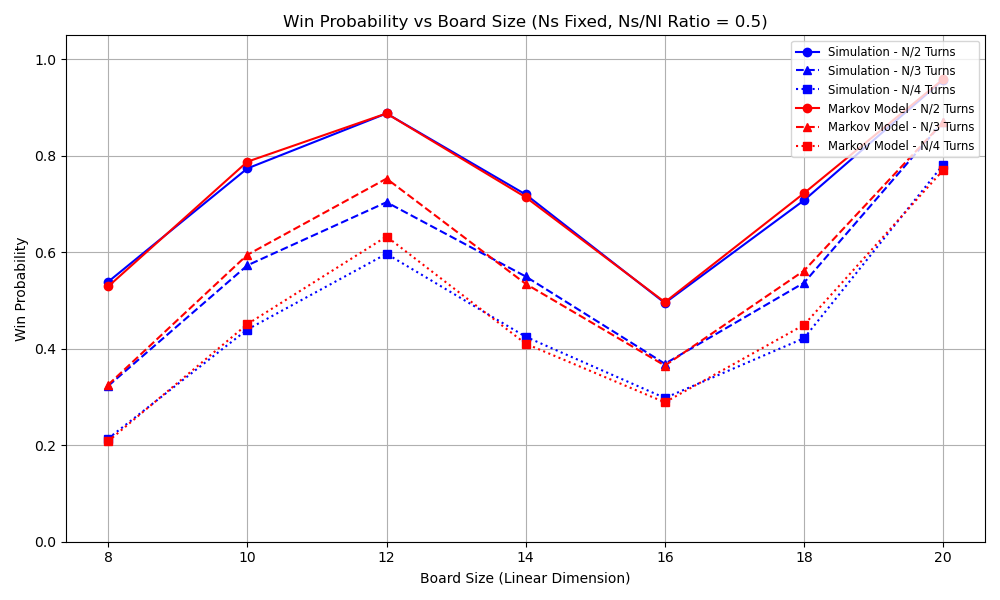
\includegraphics[width=0.8\textwidth]{"../Markov Modelling/Code/plots/plots/chapter4_validation/win_probability_plot_NsFixed_05.png"}
	\caption{\textbf{Win Probability vs Board Size} Comparison of win probabilities within $\frac{\text{BoardSize}}{2}$, $\frac{\text{BoardSize}}{3}$, and $\frac{\text{BoardSize}}{4}$ turns, derived from agent-based simulations and Markov model predictions, demonstrating a high degree of agreement.}
	\label{fig:winprobability_NsFixed_05}
\end{figure}

As illustrated in Figure \ref{fig:winprobability_NsFixed_05}, the Markov model's predictions for win probabilities closely align with the empirical results from agent-based simulations. Both methodologies demonstrate a similar trend: win probabilities within limited turns generally \textit{increase} as board size expands, despite the longer average game durations associated with larger boards, as discussed in Chapter 3.  This counter-intuitive finding, validated by both simulation and analytical methods, underscores the impact of board size on game dynamics. The close agreement between the predicted and simulated probabilities extends the confidence in our implementation of the Markov model; Its ability to capture essential aspects of game difficulty impacting beyond just the average game duration and by extension the enjoyment.  Further comparisons across other $\frac{N_s}{N_l}$ ratios and density configurations would similarly strengthen this validation.

\subsection{Comparative Distribution Analysis: Game Turns}

A more granular validation of the Markov model is achieved by comparing the full distribution of game turns. Figure \ref{fig:frequencydistributionMarkov} presents a comparative view of a particular configuration's turn distributions. Here, the turn distribution displays the probabilities of winning in certain number of turns by juxtaposing empirical distributions from 10,000 agent-based simulations against the distribution derived from the Markov model. The Markov-derived distribution is generated by probabilistically simulating\footnote{The computations were implemented in Python 3.13.2 \autocite{python}} game  progression through the transition matrix for 10,000 iterations, mirroring the simulation approach.

\begin{figure}[th]
	\centering
	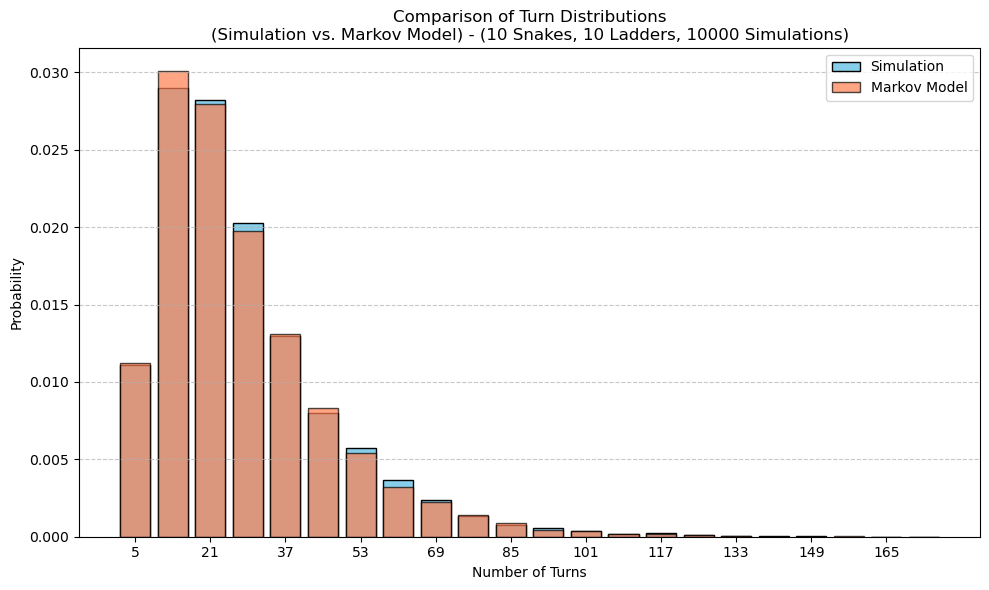
\includegraphics[width=0.8\textwidth]{"../Markov Modelling/Data/FrequencyOveralyed.png"}
	\caption{\textbf{Distribution of Game Turns: Simulation vs. Markov Model (10 Snakes, 10 Ladders, 10,000 Games):} Probability distributions of game turns from agent-based simulations and Markov model-based predictions exhibit a high degree of congruence, demonstrating model validity.}
	\label{fig:frequencydistributionMarkov}
\end{figure}

Visual inspection of Figure \ref{fig:frequencydistributionMarkov} indicates a strong qualitative agreement between the two distributions. Both exhibit a characteristic right-skewed pattern, peaking in the 10-20 turn range and displaying a long tail extending towards higher turn counts. This near identical mirroring of the turns taken to achieve a victory indicates the efficacy of the model at being able to replicate the results from empirical observations. It shows, that the model is able to accurately capture the game's characteristics and is flexible enough to accommodate changes and effectively see their effects on the metrics such as Average duration of a game \autocite{althoenHowLongGame1993a}.

This close mirroring of distributional shapes and central tendencies provides compelling evidence that the Markov model accurately captures the stochasticity and overall dynamics of game progression in Snakes and Ladders. The histogram derived from agent-based simulations closely aligns with the distribution predicted by the Markov model, further solidifying the model's capacity to represent the game's probabilistic nature.

\subsection{Steady-State Distribution and Gameplay Hotspots}
A steady-state distribution, is a probability distribution that remains unchanged over time, i.e. the probability of being in each state converges to a fixed value, regardless of the initial state. A Markov chain has a unique steady-state distribution if every state is reachable from every other state and is aperiodic (i.e. it doesn't go through a set of states with only a fixed period of validity) \autocite{mcgregorCMPSCI240Reasoning}.
 
The steady-state distribution, derived analytically from our Markov model, offers insights into the long-term probabilities of tile occupation, representing the equilibrium state of the game over infinite plays. Figure \ref{fig:steady_state_heatmap_chapter3} visualises this steady-state distribution as a heatmap.
\begin{figure}[ht]
	\centering
	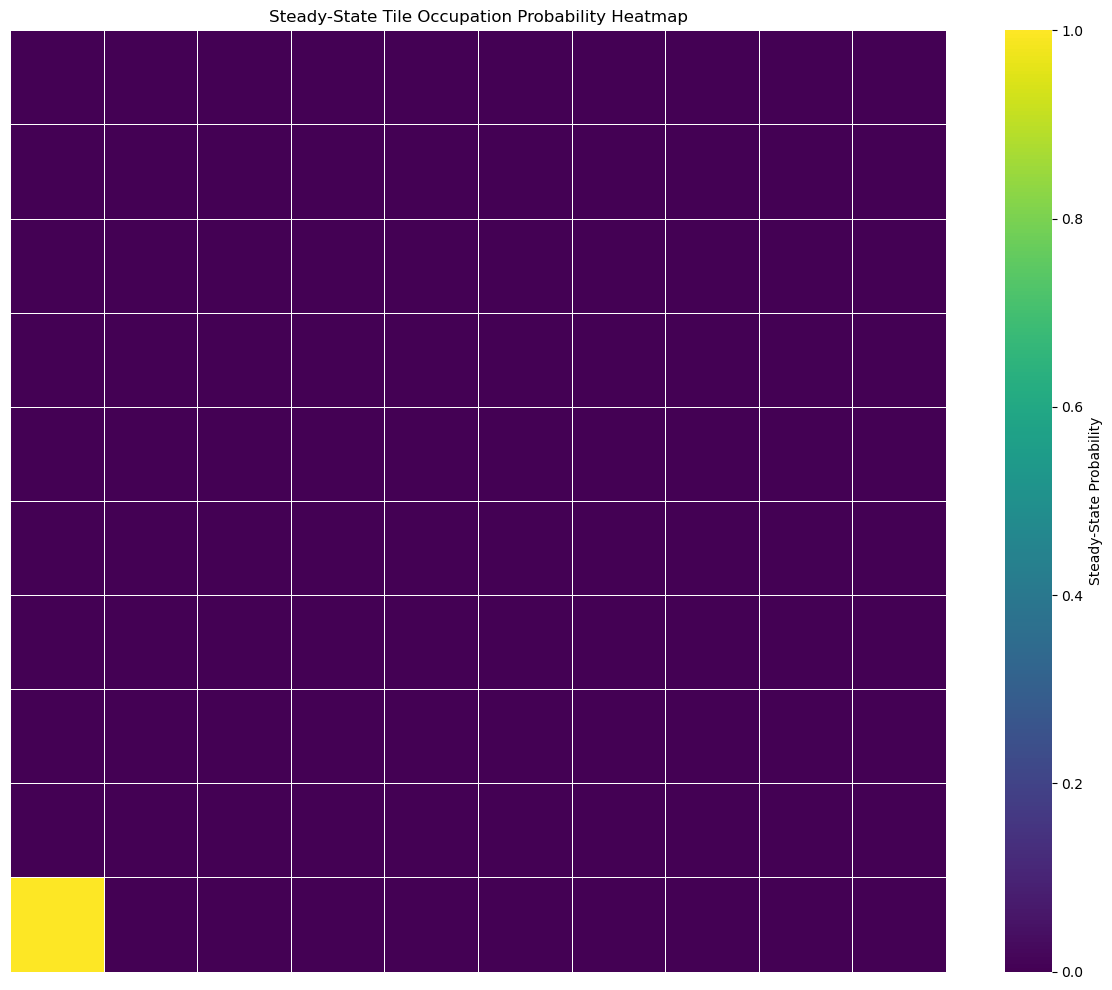
\includegraphics[width=0.6\textwidth]{"../Markov Modelling/Data/SteadyStateHeatmap.png"}
	\caption{\textbf{Steady-State Heatmap:} From Markov Model, illustrating long-term equilibrium.}
	\label{fig:steady_state_heatmap_chapter3}
\end{figure}

As theoretically expected for a well-formulated absorbing Markov chain, the Steady-State Heatmap (Figure \ref{fig:steady_state_heatmap_chapter3} demonstrates a probability of 1.0 concentrated on tile 100 (bottom-right corner), with probabilities for all other tiles approaching zero. This analytically confirms that, in the long run, the game predictably terminates at the absorbing winning state.

\subsection{Analytical Efficiency in Game Duration Derivation}

A significant advantage of the Markov model is its analytical efficiency in deriving expected game duration. Unlike agent-based simulations, which require computationally intensive repeated trials to approximate average game durations, the Markov model offers a direct, deterministic calculation through fundamental matrix analysis. This analytical solution provides a rigorous and computationally efficient alternative for determining average game durations across diverse board configurations and parameter settings. The demonstrated close agreement between the analytical expected turns and simulation-based average turns validates the Markovian approach as not only accurate but also a computationally advantageous tool for analysing game duration in Snakes and Ladders.

\section{Conclusion: Validation and Utility of the Markov Model}

This chapter has successfully constructed a Markov Chain model for Snakes and Ladders. By comparing our findings across the prior chapters, encompassing expected game duration, win probabilities, game turn distributions, and steady-state behaviour, we have observed a clear convergence between the predictions of the Markov model and the empirical findings from agent-based simulations. And finally, in the next chapter, we conclude this dissertation by assessing the collective insights we have gained throughout this dissertation. 